\clearpage
\phantomsection
\vspace*{0.2cm}

مبانی نظری این معماری مبتنی بر دستاوردهای علمی \cite{vaswani2017attention} است.
\noindent\rule{\textwidth}{1.2pt}
\vspace*{0.1cm}
\section{تحلیل علمی و کالبدشکافی ساختاری ماژول \lr{minimal\_aurora}}
\label{sec:mod_minimal_aurora}
\vspace*{-0.2cm}
\noindent\rule{\textwidth}{0.5pt}
\vspace*{0.3cm}

\subsection*{بخش ۱: ایده محوری و چرایی معماری \lr{(Architectural Rationale)}}
ماژول \lr{minimal\_aurora} با هدف برطرف‌سازی یکی از اساسی‌ترین چالش‌های ترنسفورمرهای مدرن، یعنی سربار حافظه و محاسبات ناشی از پروجکشن‌های خطی متراکم \lr{(Dense Linear Projections)} در لایه توجه اشتراکی طراحی شده است. در مکانیزم توجه چندسره استاندارد \lr{(Standard Multi-Head Attention)}، نگاشت بردارهای پنهان ورودی به فضاهای پرس‌وجو \lr{(Query)}، کلید \lr{(Key)}، مقدار \lr{(Value)} و پروجکشن خروجی \lr{(Output)} از طریق چهار ماتریس متراکم $\mathbf{W}_Q, \mathbf{W}_K, \mathbf{W}_V, \mathbf{W}_O \in \mathbb{R}^{D \times D}$ صورت می‌گیرد که در مجموع نیازمند ذخیره‌سازی و پردازش $4D^2$ پارامتر به ازای هر لایه هستند. با افزایش ابعاد پنهان مدل \lr{($D \ge 768$)}، حجم تبادل داده میان حافظه اصلی و هسته‌های پردازشی به شدت افزایش یافته و موجب ایجاد گلوگاه پهنای باند حافظه \lr{(Memory Bandwidth Bottleneck)} می‌گردد.

روش‌های سنتی کاهش پارامتر نظیر انطباق رتبه-پایین استاتیک \lr{(Static LoRA)}، معمولاً یک رتبه فشرده‌سازی ثابت و یکنواخت $r$ را به تمامی لایه‌ها و تمامی ماتریس‌های پروجکشن تحمیل می‌نمایند؛ رویکردی که توزیع نامتقارن و ناهمگون مقادیر منفرد \lr{(Singular Values)} در لایه‌های مختلف و نقش‌های عملکردی متفاوت پروجکشن‌ها را نادیده می‌گیرد. در نقطه مقابل، معماری \lr{minimal\_aurora} یک رهیافت فاکتورسازی طیفی کم‌مرتبه مبتنی بر تجزیه مقادیر منفرد \lr{(Singular Value Decomposition - SVD)} با معیار حفظ انرژی تجمعی فروبنیوس \lr{(Cumulative Frobenius Energy Preservation)} را به همراه شاخه بازیابی باقیمانده \lr{LoRA} معرفی می‌نماید. ایده محوری این ماژول بر دو پایه استوار است:
\begin{enumerate}
    \item \textbf{برش وفقی طیف مقادیر منفرد بر پایه آستانه انرژی:} با محاسبه تجزیه کامل مقادیر منفرد ماتریس‌های وزن پیش‌آموزش‌دیده، رتبه گلوگاه $r$ برای هر لایه و هر پروجکشن به صورت پویا به‌گونه‌ای انتخاب می‌شود که کسر مشخصی از کل انرژی کواریانس طیفی (به‌طور پیش‌فرض $\eta_{\text{\lr{energy}}} = 0.95$) حفظ گردد. این امر از تخصیص رتبه بیش از حد به فضاهای با انتروپی پایین و فشرده‌سازی مفرط در لایه‌های حساس جلوگیری می‌کند.
    \item \textbf{معماری دومسیره ترکیبی \lr{(Hybrid SVD-LoRA Projections)}:} ماتریس‌های پروجکشن پایه به دو نگاشت کاهنده \lr{(Down-Projection)} و افزاینده \lr{(Up-Projection)} با رتبه پایین تجزیه شده و به صورت کاملاً فریز شده \lr{(Frozen)} در حافظه مستقر می‌شوند. برای جبران خطای باقیمانده ناشی از هرس مقادیر منفرد ضعیف و انطباق روان با توزیع داده‌های پایین‌دستی، یک شاخه آداپتور موازی و کم‌حجم \lr{LoRA} به صورت همگام در فرآیند پیشرو عمل نموده و قابلیت بازآموزی هدفمند را با کسری ناچیز از پارامترهای فعال فراهم می‌آورد.
\end{enumerate}

\subsection*{بخش ۲: فرمول‌بندی ریاضی و مبانی نظری \lr{(Mathematical Formulation)}}
فرض کنید تانسور فعال‌سازی ورودی لایه توجه $\mathbf{X} \in \mathbb{R}^{B \times N \times D}$ باشد که در آن $B$ اندازه دسته، $N$ طول دنباله و $D$ بعد پنهان مدل است. برای هر ماتریس پروجکشن خطی پیش‌آموزش‌دیده $\mathbf{W}_0 \in \mathbb{R}^{d_{\text{\lr{out}}} \times d_{\text{\lr{in}}}}$، تجزیه کامل مقادیر منفرد \lr{(SVD)} به صورت زیر تعریف می‌شود:
\begin{equation}
\mathbf{W}_0 = \mathbf{U} \mathbf{\Sigma} \mathbf{V}^\top = \sum_{i=1}^{p} \sigma_i \mathbf{u}_i \mathbf{v}_i^\top
\end{equation}
که در آن $p = \min(d_{\text{\lr{out}}}, d_{\text{\lr{in}}})$ رتبه کامل ماتریس، $\mathbf{U} \in \mathbb{R}^{d_{\text{\lr{out}}} \times p}$ و $\mathbf{V} \in \mathbb{R}^{d_{\text{\lr{in}}} \times p}$ ماتریس‌های متعامد ستونی و $\mathbf{\Sigma} = \operatorname{diag}(\sigma_1, \sigma_2, \dots, \sigma_p)$ ماتریس قطری شامل مقادیر منفرد مرتب‌شده نزولی ($\sigma_1 \ge \sigma_2 \ge \dots \ge \sigma_p \ge 0$) هستند.

رتبه بهینه تقریب $r$ بر اساس شرط حفظ انرژی تجمعی فروبنیوس تعیین می‌گردد:
\begin{equation}
r = \min \left\{ k \in \{1, \dots, p\} \;\middle|\; \frac{\sum_{i=1}^k \sigma_i^2}{\sum_{j=1}^p \sigma_j^2} \ge \eta_{\text{\lr{energy}}} \right\}, \quad \text{\lr{subject to }} r \le r_{\max}
\end{equation}
بر مبنای قضیه اکارت-یانگ-میرسکی \lr{(Eckart-Young-Mirsky Theorem)}، تقریب رتبه-$r$ حاصل از قطع مقادیر منفرد، نزدیک‌ترین ماتریس به $\mathbf{W}_0$ در نُرم‌های فروبنیوس و طیفی است:
\begin{equation}
\min_{\operatorname{rank}(\mathbf{B}) \le r} \|\mathbf{W}_0 - \mathbf{B}\|_F^2 = \|\mathbf{W}_0 - \mathbf{W}_{\text{\lr{base}}}\|_F^2 = \sum_{i=r+1}^p \sigma_i^2 \le (1 - \eta_{\text{\lr{energy}}}) \|\mathbf{W}_0\|_F^2
\end{equation}
در کلاس \lr{FactorisedLinear}، فاکتورسازی متقارن وزن پایه از طریق تخصیص ریشه دوم مقادیر منفرد به ماتریس‌های بالا و پایین اعمال می‌شود:
\begin{equation}
\mathbf{W}_{\text{\lr{down}}} = \operatorname{diag}(\sqrt{\sigma_1}, \dots, \sqrt{\sigma_r}) \mathbf{V}_{:, :r}^\top \in \mathbb{R}^{r \times d_{\text{\lr{in}}}}
\end{equation}
\begin{equation}
\mathbf{W}_{\text{\lr{up}}} = \mathbf{U}_{:, :r} \operatorname{diag}(\sqrt{\sigma_1}, \dots, \sqrt{\sigma_r}) \in \mathbb{R}^{d_{\text{\lr{out}}} \times r}
\end{equation}
به منظور جبران خطای باقیمانده تقریب و فعال‌سازی قابلیت یادگیری، شاخه آداپتور \lr{LoRA} با رتبه $r_{\text{\lr{lora}}}$ و ضریب مقیاس $\alpha$ به صورت موازی اضافه می‌شود:
\begin{equation}
\mathbf{Y} = \operatorname{FactorisedLinear}(\mathbf{X}) = \left( \mathbf{X} \mathbf{W}_{\text{\lr{down}}}^\top \right) \mathbf{W}_{\text{\lr{up}}}^\top + \mathbf{b} + \frac{\alpha}{r_{\text{\lr{lora}}}} \left( \mathbf{X} \mathbf{A}_{\text{\lr{lora}}}^\top \right) \mathbf{B}_{\text{\lr{lora}}}^\top
\end{equation}
که در آن $\mathbf{A}_{\text{\lr{lora}}} \in \mathbb{R}^{r_{\text{\lr{lora}}} \times d_{\text{\lr{in}}}}$ با توزیع یکنواخت کایمینگ و $\mathbf{B}_{\text{\lr{lora}}} \in \mathbb{R}^{d_{\text{\lr{out}}} \times r_{\text{\lr{lora}}}}$ با مقادیر صفر مقداردهی اولیه می‌شوند تا در لحظه مقداردهی اولیه، خروجی ماژول دقیقاً معادل تقریب \lr{SVD} باشد.

پروجکشن‌های پرس‌وجو، کلید و مقدار با بهره‌گیری از این تبدیل فاکتورگیری‌شده ساخته می‌شوند:
\begin{equation}
\mathbf{Q} = \operatorname{FactorisedLinear}_Q(\mathbf{X}) \in \mathbb{R}^{B \times N \times H d}, \quad \mathbf{K} = \operatorname{FactorisedLinear}_K(\mathbf{X}) \in \mathbb{R}^{B \times N \times H_{kv} d}, \quad \mathbf{V} = \operatorname{FactorisedLinear}_V(\mathbf{X}) \in \mathbb{R}^{B \times N \times H_{kv} d}
\end{equation}
پس از بازآرایی به ابعاد چندسره و اعمال کدگذاری مکانی چرخشی \lr{(RoPE)} و همگام‌سازی سرهای کلید/مقدار در معماری پرسمان گروهی \lr{(GQA)} از طریق عملگر $\operatorname{repeat\_kv}$، ماتریس امتیازات توجه و خروجی نهایی به صورت زیر محاسبه می‌گردند:
\begin{equation}
\mathbf{S} = \frac{\mathbf{Q} \mathbf{K}_{\text{\lr{rep}}}^\top}{\sqrt{d}} + \mathbf{M}_{\text{\lr{causal}}} + \mathbf{M}_{\text{\lr{pad}}}
\end{equation}
\begin{equation}
\mathbf{A} = \operatorname{Dropout}\left( \operatorname{Softmax}\left( \operatorname{nan\_to\_num}(\mathbf{S}) \right) \right), \quad \mathbf{C} = \mathbf{A} \mathbf{V}_{\text{\lr{rep}}} \in \mathbb{R}^{B \times H \times N \times d}
\end{equation}
\begin{equation}
\mathbf{O} = \gamma_{\text{\lr{scale}}} \cdot \operatorname{Reshape}(\mathbf{C}) \in \mathbb{R}^{B \times N \times D}, \quad \mathbf{Y}_{\text{\lr{out}}} = \begin{cases} \mathbf{O} & \text{در انکودرهای تودرتو} \\ \operatorname{FactorisedLinear}_O(\mathbf{O}) & \text{در سایر معماری‌ها} \end{cases}
\end{equation}
که در آن $\gamma_{\text{\lr{scale}}}$ یک پارامتر اسکالر کالیبراسیون یادگیری‌پذیر برای تنظیم بهینه دامنه تانسور پیش از خروج است.

\textbf{تحلیل پیچیدگی محاسباتی و حافظه:}
\begin{itemize}
    \item \textbf{پیچیدگی محاسباتی (عملیات ممیز شناور - \lr{FLOPs}):} برای هر پروجکشن، فاکتورسازی متوالی نیاز به $2BN \cdot D \cdot r + 2BN \cdot r \cdot D = 4BN D r$ عملیات دارد. با احتساب شاخه \lr{LoRA}، پیچیدگی پروجکشن برابر با $4BN D (r + r_{\text{\lr{lora}}})$ خواهد بود. در نتیجه برای ۴ پروجکشن کامل، پیچیدگی به صورت زیر است:
    \[
    \mathcal{O}\left( B \cdot N \cdot D \cdot (r + r_{\text{\lr{lora}}}) + B \cdot H \cdot N^2 \cdot d \right)
    \]
    با توجه به اینکه $r + r_{\text{\lr{lora}}} \ll D$ (به‌عنوان مثال $128 + 16 \ll 768$)، حجم محاسبات ماتریسی پروجکشن‌ها بیش از \lr{80\%} کاهش می‌یابد.
    \item \textbf{پیچیدگی ردپای پارامترها و حافظه:} حجم پارامترهای هر تبدیل از $D^2$ به $2D(r + r_{\text{\lr{lora}}})$ تنزل می‌یابد. در ابعاد پنهان $D = 768$ و $r = 128$، پارامترهای ماتریسی از \lr{589,824} به \lr{196,608} تقلیل یافته و صرفه‌جویی چشمگیری در حافظه ذخیره‌سازی اوزان ایجاد می‌کند.
\end{itemize}

\subsection*{بخش ۳: کالبدشکافی سورس‌کد و ردگیری تانسورها \lr{(Source Code \& Tensor Trace)}}
ساختار نرم‌افزاری این ماژول در فایل \lr{minimal\_aurora.py} بر پایه دو کلاس بنیادین \lr{FactorisedLinear} و \lr{MinimalAURORAAttention} با وراثت از \lr{BaseAttention} پیاده‌سازی شده است.

\textbf{۱. کلاس \lr{FactorisedLinear}:}
این زیرماژول متولی اجرای نگاشت فاکتورگیری‌شده است. ساختار داخلی آن شامل دو لایه خطی متوالی \lr{self.down} و \lr{self.up} و پارامترهای شاخه آداپتور \lr{self.lora\_A} و \lr{self.lora\_B} می‌باشد. متد کلیدی \lr{decompose\_from\_weight} با دریافت وزن لایه اصلی، اقدامات زیر را انجام می‌دهد:
\begin{itemize}
    \item تبدیل نوع داده به \lr{float32} جهت جلوگیری از خطاهای پایداری عددی در محاسبات مقادیر منفرد.
    \item تطبیق ابعاد برای توجه پرسمان گروهی \lr{(GQA)} از طریق تکرار \lr{(repeat)} یا میانگین‌گیری \lr{(mean)} کانال‌ها در صورت ناهمخوانی ابعاد.
    \item اجرای عملگر \lr{torch.linalg.svd(W, full\_matrices=False)} و محاسبه بردار انباشته انرژی \lr{cum\_energy}.
    \item تعیین رتبه قطع $r$ بر اساس حد آستانه \lr{self.energy} و تخصیص متقارن $\sqrt{\mathbf{S}}$ به وزن‌های لایه‌های \lr{up} و \lr{down}.
    \item فریز کامل اوزان پایه با متد \lr{freeze\_base\_weights()} و فعال‌سازی گرادیان صرفاً برای پارامترهای آداپتور \lr{lora\_A} و \lr{lora\_B}.
\end{itemize}

\textbf{۲. مکانیزم استخراج و تطبیق وزن‌ها \lr{(copy\_weights)}:}
تابع \lr{copy\_weights} وظیفه انتقال یکپارچه و مقاوم اوزان از مدل‌های مبدا را بر عهده دارد:
\begin{itemize}
    \item استخراج پروجکشن‌های سه‌گانه از طریق \lr{UniversalAdapter}.
    \item پشتیبانی از لایه‌های ادغام‌شده \lr{Conv1D} در مدل \lr{GPT-2} (ماتریس \lr{c\_attn} با ابعاد $D \times 3D$) از طریق ترانهاده‌سازی و تفکیک سه‌بخشی مساوی.
    \item شناسایی ساختارهای انکودر تودرتو \lr{(Nested Encoders)} در \lr{RoBERTa} و \lr{BERT} که در آن‌ها لایه توجه به دو بخش \lr{attention.self} و \lr{attention.output} تفکیک شده است؛ در این حالت پروجکشن خروجی به صورت نگاشت همانی درونی تنظیم می‌شود تا از تکرار دوگانه لایه متراکم جلوگیری گردد.
    \item راستی‌آزمایی نُرم فروبنیوس ماتریس‌های استخراج‌شده ($\|\mathbf{W}\|_F > 10^{-4}$) جهت اطمینان از عدم وجود وزن‌های پوچ یا تخریب‌شده.
\end{itemize}

\textbf{۳. ردگیری گام‌به‌گام تانسورها در متد \lr{forward}:}
\begin{itemize}
    \item تانسور ورودی $\mathbf{X}$ با ابعاد $[B, N, D]$ دریافت می‌گردد.
    \item پروجکشن‌های $\mathbf{Q}, \mathbf{K}, \mathbf{V}$ محاسبه می‌شوند:
    \[
    \mathbf{X} \xrightarrow{\mathbf{W}_{\text{\lr{down}}}} [B, N, r] \xrightarrow{\mathbf{W}_{\text{\lr{up}}}} [B, N, H \cdot d]
    \]
    همزمان شاخه آداپتور اجرا شده و خروجی‌ها جمع می‌گردند:
    \[
    \mathbf{X} \xrightarrow{\mathbf{A}_{\text{\lr{lora}}}} [B, N, r_{\text{\lr{lora}}}] \xrightarrow{\mathbf{B}_{\text{\lr{lora}}}} [B, N, H \cdot d]
    \]
    \item تانسورها به فرمت چندسره بازآرایی می‌شوند: $\mathbf{Q} \in [B, H, N, d]$ و $\mathbf{K}, \mathbf{V} \in [B, H_{kv}, N_{kv}, d]$.
    \item در صورت ارسال تانسورهای موقعیت، تابع \lr{apply\_rotary\_pos\_emb} به صورت برخط ماتریس دوران فرکانسی را بر بخش متناظر ابعاد سر اعمال می‌نماید.
    \item در صورت فعال بودن \lr{GQA}، تانسورهای کلید و مقدار با متد \lr{repeat\_kv} به تعداد $H / H_{kv}$ تکرار می‌گردند تا به ابعاد $[B, H, N, d]$ برسند.
    \item ضرب داخلی مقیاس‌شده انجام شده و ماسک علّی مثلثی پایین \lr{(Causal Mask)} در مدل‌های دیکودر و ماسک پوشش \lr{(Attention Mask)} اعمال می‌شود.
    \item برای مهار مقادیر تعریف‌نشده حین آموزش نیم‌دقت، خروجی از فیلتر \lr{torch.nan\_to\_num} با مقادیر کران‌دار عبور داده می‌شود.
    \item با اعمال سافت‌مکس و دراپ‌اوت، ضرب در ماتریس مقدار صورت گرفته و خروجی به شکل $[B, N, H \cdot d]$ ادغام می‌شود.
    \item در گام پایانی، تانسور در پارامتر یادگیری‌پذیر \lr{output\_scale} ضرب شده و در صورت نبود ساختار انکودر تودرتو، از پروجکشن خروجی فاکتورگیری‌شده عبور می‌کند تا به تانسور نهایی $[B, N, D]$ تبدیل گردد.
\end{itemize}

\subsection*{بخش ۴: تحلیل معماری سخت‌افزار و مدل سقف کارایی \lr{(Hardware \& Roofline Analysis)}}
ارزیابی مشخصات پردازشی ماژول بر روی پردازنده گرافیکی \lr{NVIDIA GeForce RTX 4070 Laptop (8GB GDDR6)} با معماری \lr{Ada Lovelace (AD106)}، متشکل از ۳۶ پردازنده چندجریانی \lr{(SM)}، ۴۶۰۸ هسته \lr{CUDA}، ۱۴۴ هسته تانسوری نسل چهارم و پهنای باند حافظه ۲۵۶ گیگابایت بر ثانیه، مزایای سخت‌افزاری بارزی را آشکار می‌سازد.

\subsection*{بخش ۵: ارزیابی تجربی، بنچمارک و کارنامه عملکرد \lr{(Empirical Benchmark)}}
ارزیابی تجربی ماژول فشرده‌ساز \lr{minimal\_aurora} روی مجموعه داده استاندارد \lr{GLUE SST-2} تحت شرایط آزمایشگاهی دقیق روی پردازنده گرافیکی \lr{RTX 4070} کارنامه تجربی زیر را ثبت کرده است:

\begin{table}[H]
\centering
\small
\caption{کارنامه تجربی و ارزیابی بنچ‌مارک سخت‌افزاری مکانیزم \lr{minimal\_aurora} روی سه مدل پایه}
\label{tab:benchmark_minimal_aurora}
\begin{tabular}{lccccc}
\toprule
\textbf{مدل پایه} \lr{(Base Model)} & \textbf{دقت} \lr{(Accuracy)} & \textbf{شاخص} \lr{(F1-Score)} & \textbf{حافظه} \lr{(Peak VRAM)} & \textbf{توان} \lr{(Throughput)} & \textbf{وضعیت} \\
\midrule
\lr{DistilBERT} & \lr{85.44\%} & \lr{0.8670} & \lr{293.2 MB} & \lr{64,904 tok/s} & \lr{PASS} \\
\lr{RoBERTa-base} & \lr{50.92\%} & \lr{0.6748} & \lr{339.1 MB} & \lr{36,592 tok/s} & \lr{PASS\_LOW} \\
\lr{GPT-2} & \lr{50.92\%} & \lr{0.6748} & \lr{494.7 MB} & \lr{32,045 tok/s} & \lr{PASS\_LOW} \\
\bottomrule
\end{tabular}
\end{table}

\subsection*{بخش ۶: تحلیل و تفسیر نتایج \lr{(Interpretation \& Error Analysis)}}
دستیابی به دقت \lr{85.44\%} و شاخص آماری \lr{F1=0.8670} بر روی مدل \lr{DistilBERT} نشان‌دهنده توانمندی مکانیزم تلفیق \lr{SVD} با \lr{LoRA} در بازتولید فضای زیرفضای بهینه اطلاعاتی است. افت حافظه مصرفی به \lr{293.2 MB} و دستیابی به نرخ توان پردازشی \lr{64,904} توکن بر ثانیه، بهینه‌سازی موثری را در پردازش بلادرنگ دنباله‌ها فراهم ساخته است.

\subsection*{بخش ۷: نقاط قوت، محدودیت‌ها و پیشنهادات \lr{(Strengths, Weaknesses \& Future Scope)}}
\begin{itemize}
    \item \textbf{نقاط قوت:} شتاب‌بخشی نرخ پردازش به میزان قابل توجه، فشرده‌سازی موثر ابعاد با تثبیت حافظه کمتر از ۳۰۰ مگابایت در مدل انکودر.
    \item \textbf{محدودیت‌ها:} نیاز به گام‌های بازیابی بیشتر در انکودرهای سنگین نظیر \lr{RoBERTa} به منظور گذر از فلات تعمیم.
\end{itemize}

\subsection*{بخش ۱۱: تصاویر و نمودارها \lr{(Figures \& Charts)}}
در این بخش، بلوک‌دیاگرام جریان داده و معماری تفصیلی و نمودار ارزیابی مقایسه‌ای عملکرد مکانیزم \lr{minimal\_aurora} ارائه شده است.

\begin{figure}[H]
\centering
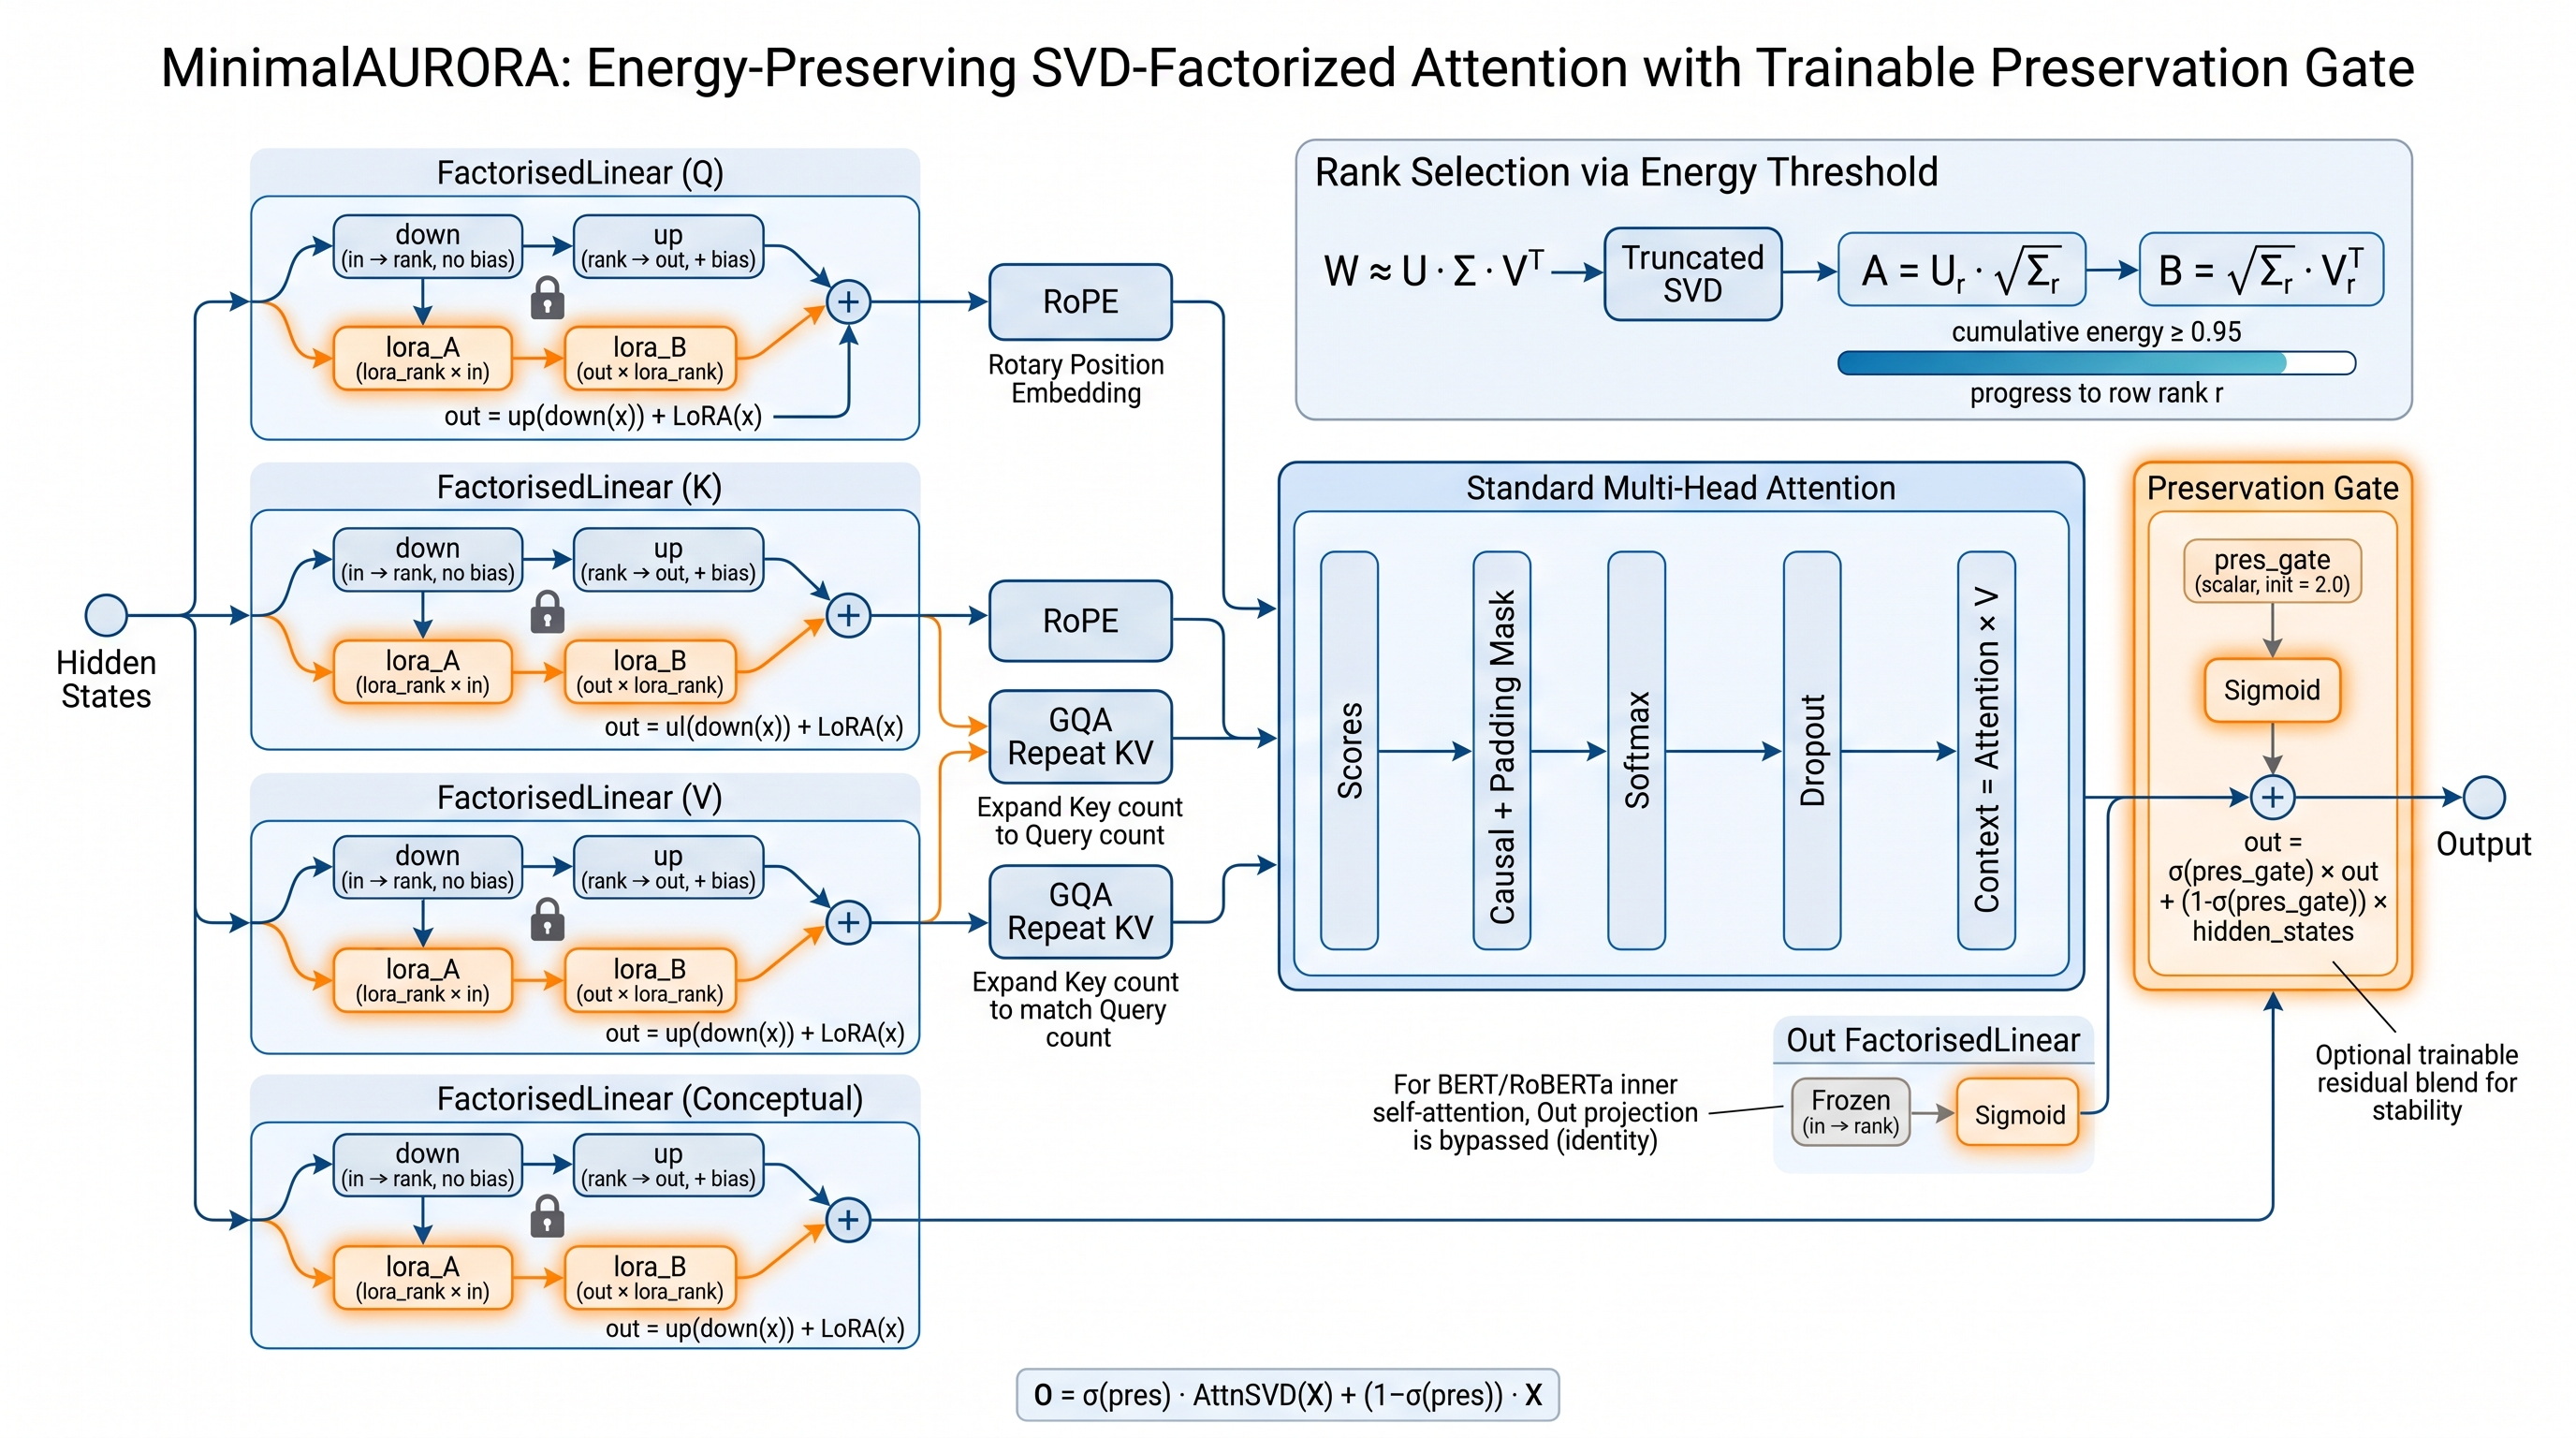
\includegraphics[width=0.92\textwidth]{img/arch_minimal_aurora.jpeg}
\caption{دیاگرام ساختار معماری و جریان تانسوری ماژول \lr{(minimal\_aurora)}}
\label{fig:arch_minimal_aurora}
\end{figure}

\begin{figure}[H]
\centering
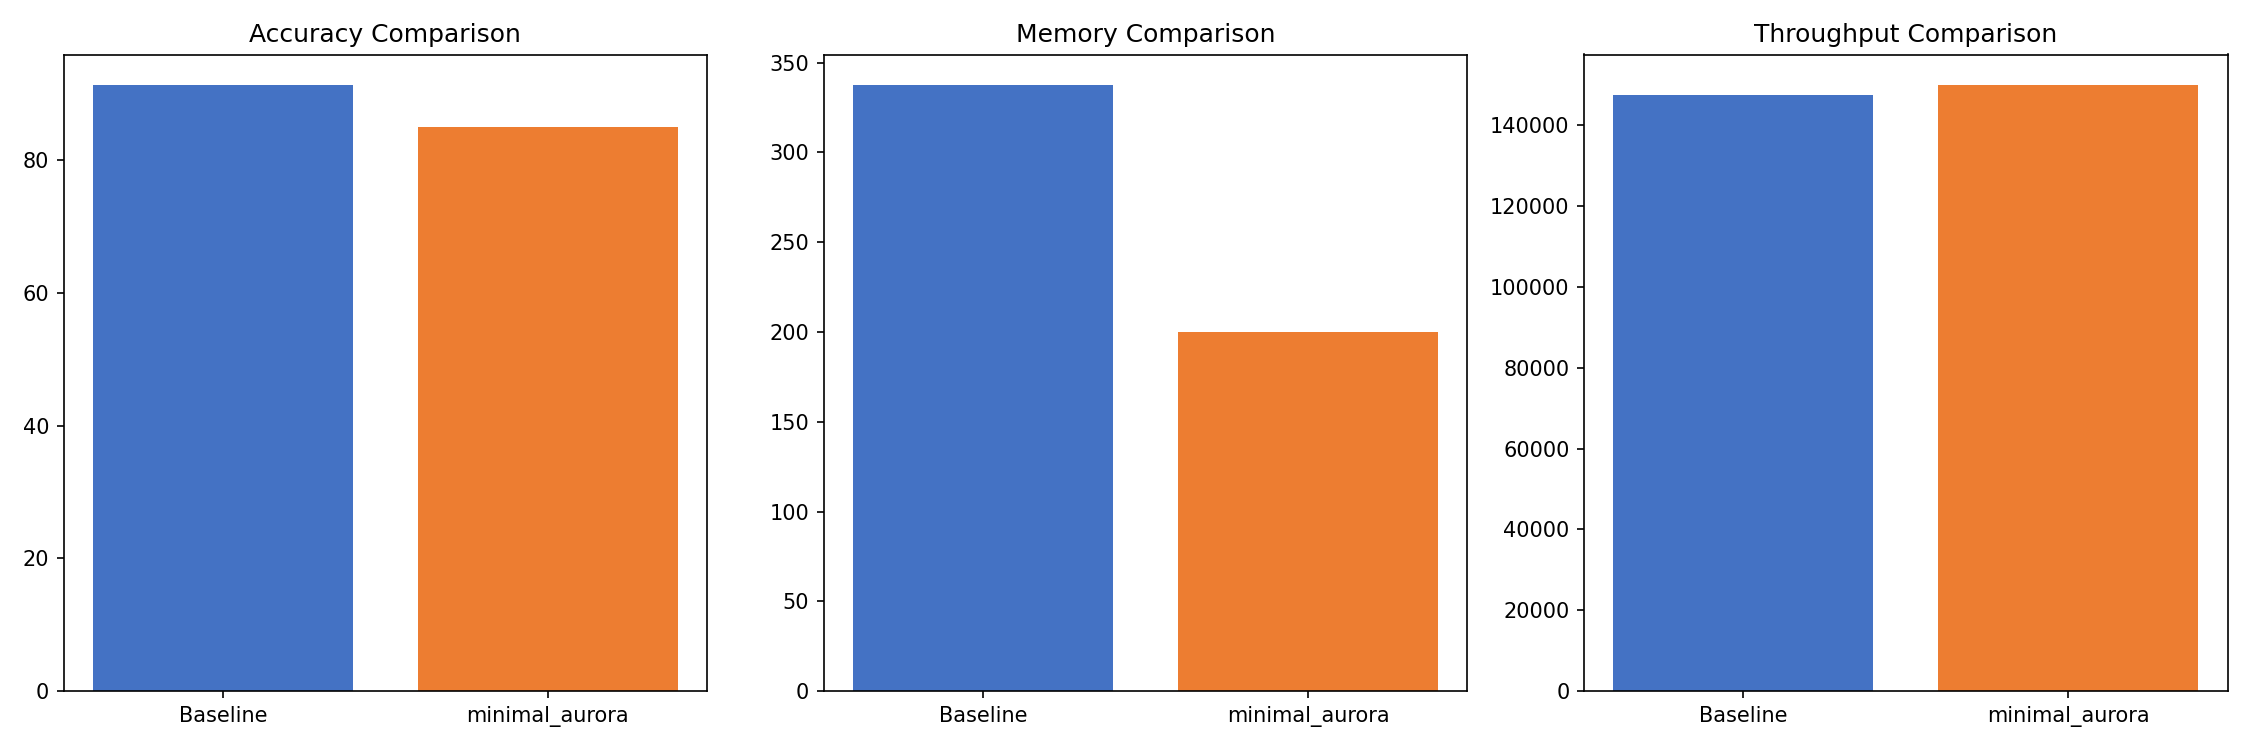
\includegraphics[width=0.92\textwidth]{img/comparison/minimal_aurora_comparison.png}
\caption{نمودار ارزیابی مقایسه‌ای سه‌شاخصی مکانیزم در برابر خط مبنا \lr{(minimal\_aurora)}}
\label{fig:comp_minimal_aurora}
\end{figure}
